\documentclass[a4paper,11pt]{article}

\usepackage[utf8]{inputenc}
\usepackage[top=2cm, left = 2cm , right=2cm , bottom=2cm]{geometry}
\usepackage{amsmath}
\usepackage{graphicx}
\usepackage{float}
\usepackage{listings}
\usepackage[brazil]{babel}

\pagestyle{plain}

\graphicspath{{./Imagens/}}

\begin{document}	

\begin{center}
\textbf{Experiência 4} \\
\hspace{5pt}
Prof. Marconi Kolm Madrid \\
EA722 - 2017/2
\end{center}

\begin{center}
Danilo Pereira Titato - RA 122541 \\
Giovani Granzotto Oliani - RA 146253 \\
Pedro Gabriel Calixto Mendonça - RA 118363 \\
\end{center}

\textbf{Exercício 1}

A função de transferência é:

\begin{gather*}
    \frac{Y\left(s\right)}{R\left(s\right)} =
        \frac{G_c\left(s\right) G_p\left(s\right)}
        {1 + G_c\left(s\right) G_p\left(s\right)}
\end{gather*}

Para o cálculo de erro:

\begin{gather*}
    Y\left(s\right) = G_c\left(s\right) \cdot G_p\left(s\right) \cdot
        E\left(s\right) \\
    \frac{G_c\left(s\right) G_p\left(s\right) E\left(s\right)}{R\left(s\right)}
        = \frac{G_c\left(s\right) G_p\left(s\right)}
        {1 + G_c\left(s\right) G_p\left(s\right)} \\
    E\left(s\right) = \frac{R\left(s\right)}
        {1 + G_c\left(s\right) G_p\left(s\right)}
\end{gather*}

Logo, o erro de estado estacionário do sistema em malha fechada é dado por:

\begin{gather*}
    e\left(\infty\right) = \lim_{s \to 0} s E\left(s\right) =
        \lim_{s \to 0} s \frac{R\left(s\right)}
        {1 + G_c\left(s\right) G_p\left(s\right)}, C.Q.D.
\end{gather*}

\textbf{Exercício 2}

Temos que, no controlador PI\&D, com $k_i = 0$:

\begin{gather*}
    X\left(s\right) = \frac{1}{m_1 s^2 + c_1 s} \cdot k_{hw} \cdot
        \left[\left(k_p + \frac{k_i}{s}\right)\left(R\left(s\right) -
        X\left(s\right)\right) - k_d s X\left(s\right)\right] \\
    X\left(s\right) \left[ 1 + \frac{1}{m_1 s^2 + c_1 s} \cdot k_{hw} \cdot
        \left(k_p + k_d s \right) \right] =
        R\left(s\right) \cdot \frac{1}{m_1 s^2 + c_1 s} \cdot k_{hw} \cdot
        k_p \\
    X\left(s\right) \left[m_1 s^2 + \left(c_1 + k_d k_{hw}\right) s +
        k_p k_{hw}\right]
        = R\left(s\right) \cdot k_p \cdot k_{hw} \\
    \frac{X\left(s\right)}{R\left(s\right)} = \frac{k_p k_{hw}}
        {m_1 s^2 + \left(c_1 + k_d k_{hw}\right) s + k_p k_{hw}}
\end{gather*}

\begin{align*}
    E\left(s\right) &= R\left(s\right) - X\left(s\right) \\
    &= R\left(s\right) \left[1 - \frac{k_p k_{hw}}
        {m_1 s^2 + \left(c_1 + k_d k_{hw}\right) s + k_p k_{hw}}\right] \\
    &= R\left(s\right) \left[\frac{m_1 s^2 + \left(c_1 + k_d k_{hw}\right) s}
        {m_1 s^2 + \left(c_1 + k_d k_{hw}\right) s + k_p k_{hw}}\right]
\end{align*}

\begin{gather*}
    e\left(\infty\right) = \lim_{s \to 0} s \cdot E\left(s\right) =
        \lim_{s \to 0} s \cdot \left[\frac{m_1 s^2 + \left(c_1 +
        k_d k_{hw}\right) s}{m_1 s^2 + \left(c_1 + k_d k_{hw}\right) s +
        k_p k_{hw}}\right], C.Q.D.
\end{gather*}

\pagebreak

Já para o controlador PD:

\begin{align*}
    \frac{X\left(s\right)}{R\left(s\right)} &= \frac{\frac{1}{m_1 s^2 + c_1 s} \cdot
        k_{hw} \cdot \left(k_p + k_d s\right)}{1 + \frac{1}{m_1 s^2 + c_1 s} \cdot
        k_{hw} \cdot \left(k_p + k_d s\right)} \\
    &= \frac{k_{hw} \cdot \left(k_p + k_d s\right)}{m_1 s^2 + \left(c_1 +
        k_d k_{hw}\right) s + k_p k_{hw}}
\end{align*}

\begin{align*}
    \widetilde{E}\left(s\right) &= R\left(s\right) - X\left(s\right) \\
    &= R\left(s\right) \cdot \left[1 - \frac{k_{hw} \cdot \left(k_p +
        k_d s\right)}{m_1 s^2 + \left(c_1 + k_d k_{hw}\right) s + k_p k_{hw}}
        \right] \\
    &= R\left(s\right) \cdot \left[\frac{m_1 s^2 + c_1 s}{m_1 s^2 + \left(c_1 +
        k_d k_{hw}\right) s + k_p k_{hw}}\right]
\end{align*}

\begin{gather*}
    \widetilde{e}\left(\infty\right) = \lim_{s \to 0} s \cdot
        \widetilde{E}\left(s\right) = \lim_{s \to 0} s \cdot
        \left[\frac{m_1 s^2 + c_1 s}{m_1 s^2 + \left(c_1 + k_d k_{hw}\right) s +
        k_p k_{hw}}\right], C.Q.D.
\end{gather*}

\textbf{Procedimento experimental - parte 1}

\textbf{2.}

\begin{figure}[H]
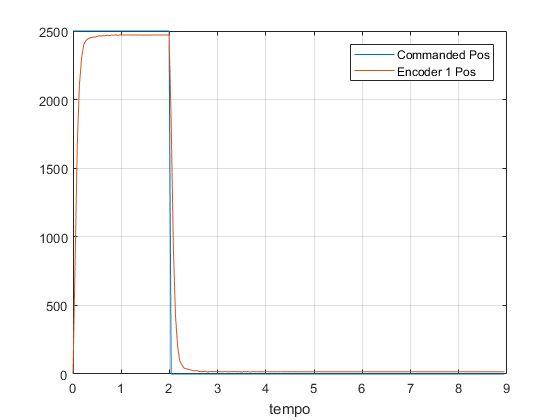
\includegraphics{q02}
\centering
\end{figure}

\pagebreak

\textbf{3.}

\begin{gather*}
    k_i k_{hw} = 7500 \implies k_i = \frac{7500}{14732} = 0.5091
\end{gather*}


\begin{figure}[H]
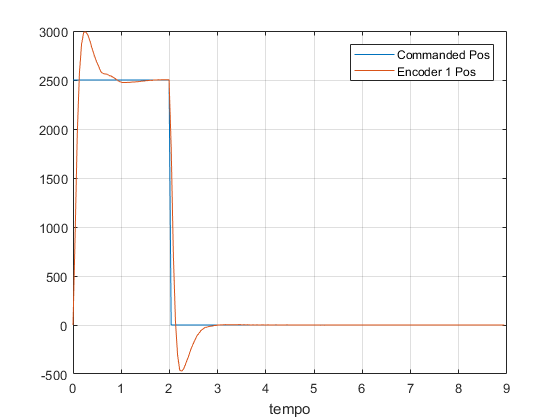
\includegraphics[scale=0.9]{q03}
\centering
\end{figure}

\textbf{4.}

\begin{figure}[H]
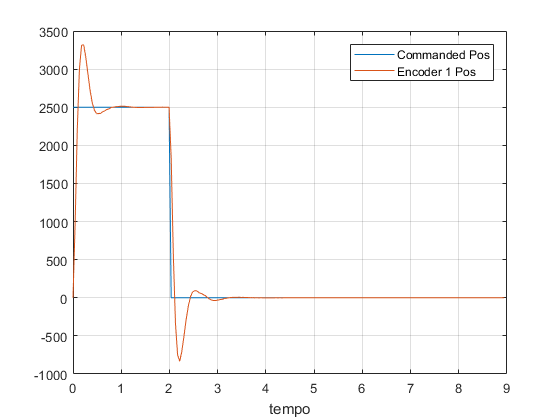
\includegraphics[scale=0.9]{q04}
\centering
\end{figure}

Como parte da força de compensação é determinada pela integral do erro; enquanto
o erro não for negativo ou zero, o termo integral aumentará de modo cumulativo.
Assim, se segurarmos o carro deslocado da origem, haverá erro e a força de
compensação irá aumentar ao longo do tempo. Se soltarmos o carro após o
segurarmos em uma posição deslocada, o carro irá acelerar em direção à posição
comandada, mas irá passar do ponto de equilíbrio e oscilar em torno dele. \\

\textbf{5.}

\begin{figure}[H]
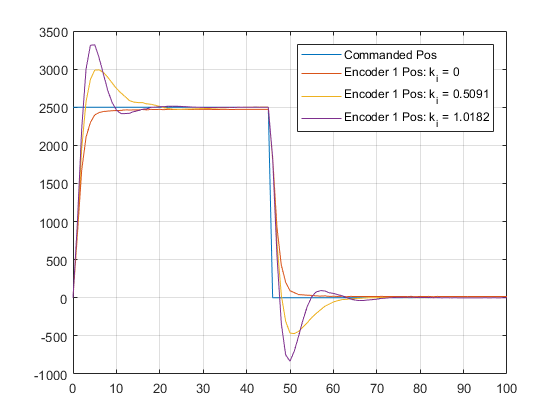
\includegraphics{q05}
\centering
\end{figure}

Como podemos ver, a ação integral elimina o erro de regime, dado que a força de
compensação aumenta enquanto houver erro. No entanto, é visível também que com
um maior ganho integral, temos um aumento visível no máximo \textit{overshoot}.
Isso pode ser explicado pelo aumento da força de compensação aplicada pelo termo
integrador, para que haja o controle ao redor do ponto de equilíbrio. Já que é
dependente do termo integrativo, essa força acumula independentemente da taxa de
variação do erro, enquanto houver erro. Com o aumento do $k_i$, há o aumento
dessa força e o sistema apresenta um \textit{overshoot} mais acentuado. \\

\pagebreak

\textbf{Procedimento experimental - parte 2}

\textbf{8.}
PI\&D, $k_i = 0$ (P\&D):

\begin{figure}[H]
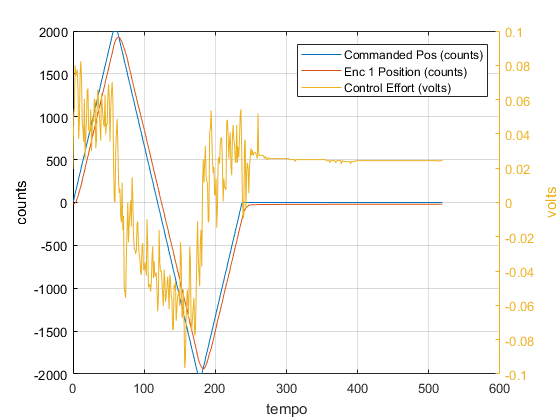
\includegraphics{q08}
\centering
\end{figure}

\textbf{9.}

PD:

\begin{figure}[H]
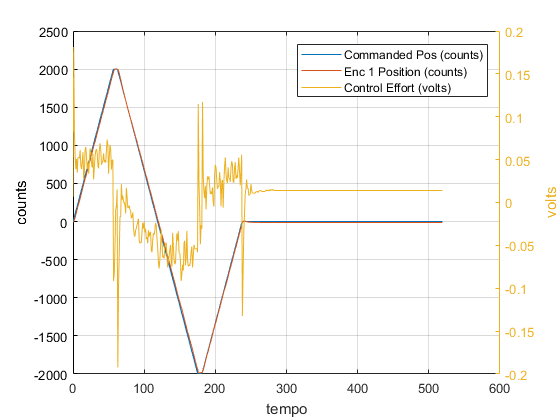
\includegraphics{q09-pd}
\centering
\end{figure}

PID:

\begin{figure}[H]
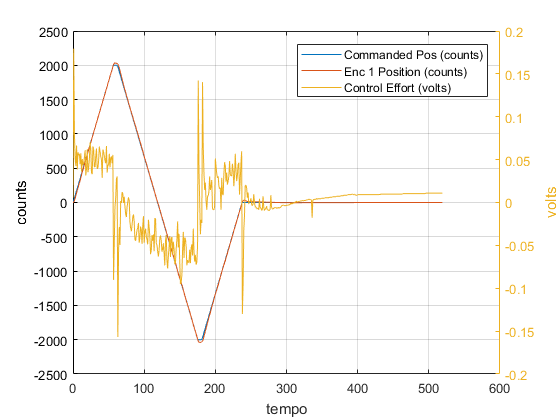
\includegraphics{q09-pid}
\centering
\end{figure}

\textbf{10.}

8-PI\&D houve erro notável, sem overshoot

9-PD existe erro mt mt mt pequeno. overshoot mt mt pequeno

9-PID houve overshoot notavel, sem erro

\textbf{Procedimento experimental - parte 3}

\textbf{12.}

\end{document}